\item In the arrangement shown in Fig. 1.18 the mass of ball 1 is \(\eta = 1.8\) times as great as that of rod 2. The length of the latter is \(l = 100\) cm. The masses of the pulleys and the threads, as well as the friction, are negligible. The ball is set on the same level as the lower end of the rod and then released. How soon will the ball be opposite the upper end of the rod?
    \begin{center}
        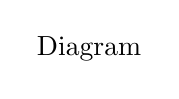
\begin{tikzpicture}
            \node at (0, 0) {Diagram};
        \end{tikzpicture}
    \end{center}
\begin{solution}
    \begin{center}
        \begin{tikzpicture}
            \pic at (0, 0) {frame=3cm};
        \end{tikzpicture}
    \end{center}

    % \begin{align*}
    %     \intertext{Suppose, the ball goes up with acceleration \( w_1 \) and the rod comes down with the acceleration \( w_2 \).}
    %     % \intertext{As the length of the thread is constant, \( 2w_1 = w_2 \) \tag{1}}
    %     \intertext{Newton’s second law in projection form, vertically upwards for the ball and vertically downwards for the rod respectively gives,}
    %     T - mg &= mw_1 \tag{2} \\
    %     Mg - T' &= Mw_2 \tag{3} \\
    %     \intertext{but, \( T = 2T' \) (because pulley is massless) }\tag{4}
    %     \intertext{From Eqs. (1), (2), (3) and (4)}
    %     w_1 &= \dfrac{(2M - m)g}{m + 4M} = \dfrac{(2 - \eta) g}{\eta + 4} \quad \text{(upwards)} \\
    %     w_2 &= \dfrac{2(2 - \eta) g}{(\eta + 4)} \quad \text{(downwards)}
    %     \intertext{From kinematical equation in projection form, we get}
    %     l &= \dfrac{1}{2} (w_1 + w_2) t^2
    %     \intertext{as \( w_1 \) and \( w_2 \) are in the opposite direction.}
    %     \intertext{Putting the values of \( w_1 \) and \( w_2 \), the sought time becomes}
    %     t &= \sqrt{\dfrac{2l (\eta + 4)/3} {(2 - \eta) g}} = 1.4 \text{ s}
    % \end{align*}
\end{solution}
